\chapter{Deep Neural Network Toolkit} 
\label{chap:toolkit}
%%%%%%%%%%%%%%%%%%%%%%%%%%%%%%%%%%%%%%%%%%%%%%%%%%%%%%%%%%%%%%%%%%%%%%%%%%%%%%%%%%%%%%%%%%%%%%%%%%%%%%%%%%%%%%%%%%%%%%%%%
\section{Introduction}
\textit{Deep Neural Networks} are the current trend in machine learning.  Deep neural networks can be best implemented using the modular, object-oriented approach. 

Even though there are many toolkits available, these toolkits lack simplicity.  Moreover the recent growth of GPU programming has paved way for fast implementation of DNN. \textit{Python-DNN} was developed with modularity and speed in mind.

\section{Python-DNN}
\textit{Python DNN} is a lightweight deep learning toolkit developed in Python, which can run on both GPU and CPU.  It makes use of \emph{theano}  \cite{bergstra2010theano} which allows optimization and evaluation of mathematical expressions involving multi-dimensional arrays efficiently.

\subsection{Existing Toolkits/libraries}
There are many toolkits and libraries have been developed for Deep Neural Network.  Some of them are: 
\begin{itemize}
\item \href{http://kaldi.sourceforge.net/}{Kaldi} \citep{Povey_ASRU2011}, a speech recognition tool-kit.
\item \href{https://github.com/rasmusbergpalm/DeepLearnToolbox}{DeepLearnToolbox} \citep{IMM2012-06284}, a toolkit for \textit{matlab \& octave}.
\item \href{http://cs.stanford.edu/people/karpathy/convnetjs/}{convnetjs} \citep{convnetjs} , a \textit{JavaScript}  based library.
\item \href{https://radimrehurek.com/gensim}{Gensim} \citep{rehurek_lrec}, a tool-kit for natural language processing.
\end{itemize}

There are many issues with these existing toolkits.  The major one is that, most of them are domain specific.  Since deep neural network is computationally heavy, there are many fast implementations of DNN, which make use of GPU.  But these toolkits work only with GPU.  None of these toolkits can work seamlessly on both GPU and multicore CPUs. 

We have built a tool-kit to overcome this problem, which can also be used as a stand-alone library


\subsection{Supported Models}
\label{sec:python-dnnModels}
\textit{Python DNN}  has support  for \textit{Deep Belief Network (DBN)} \cite{hinton2002training} (uses Restricted Boltzmann machine(RBM)), \textit{Stacked Denoising Auto-encoders (SdA)} \cite{vincent2010stacked} and \textit{Convolutional Neural Network (CNN)} \cite{lecun1998gradient} (both 2D-CNN and 3D-CNN). \textit{Python-dnn} has been developed in such a way that it can be easily extended to support other models in the future.

\subsection{Architecture}

\begin{figure}[ht]
\centering
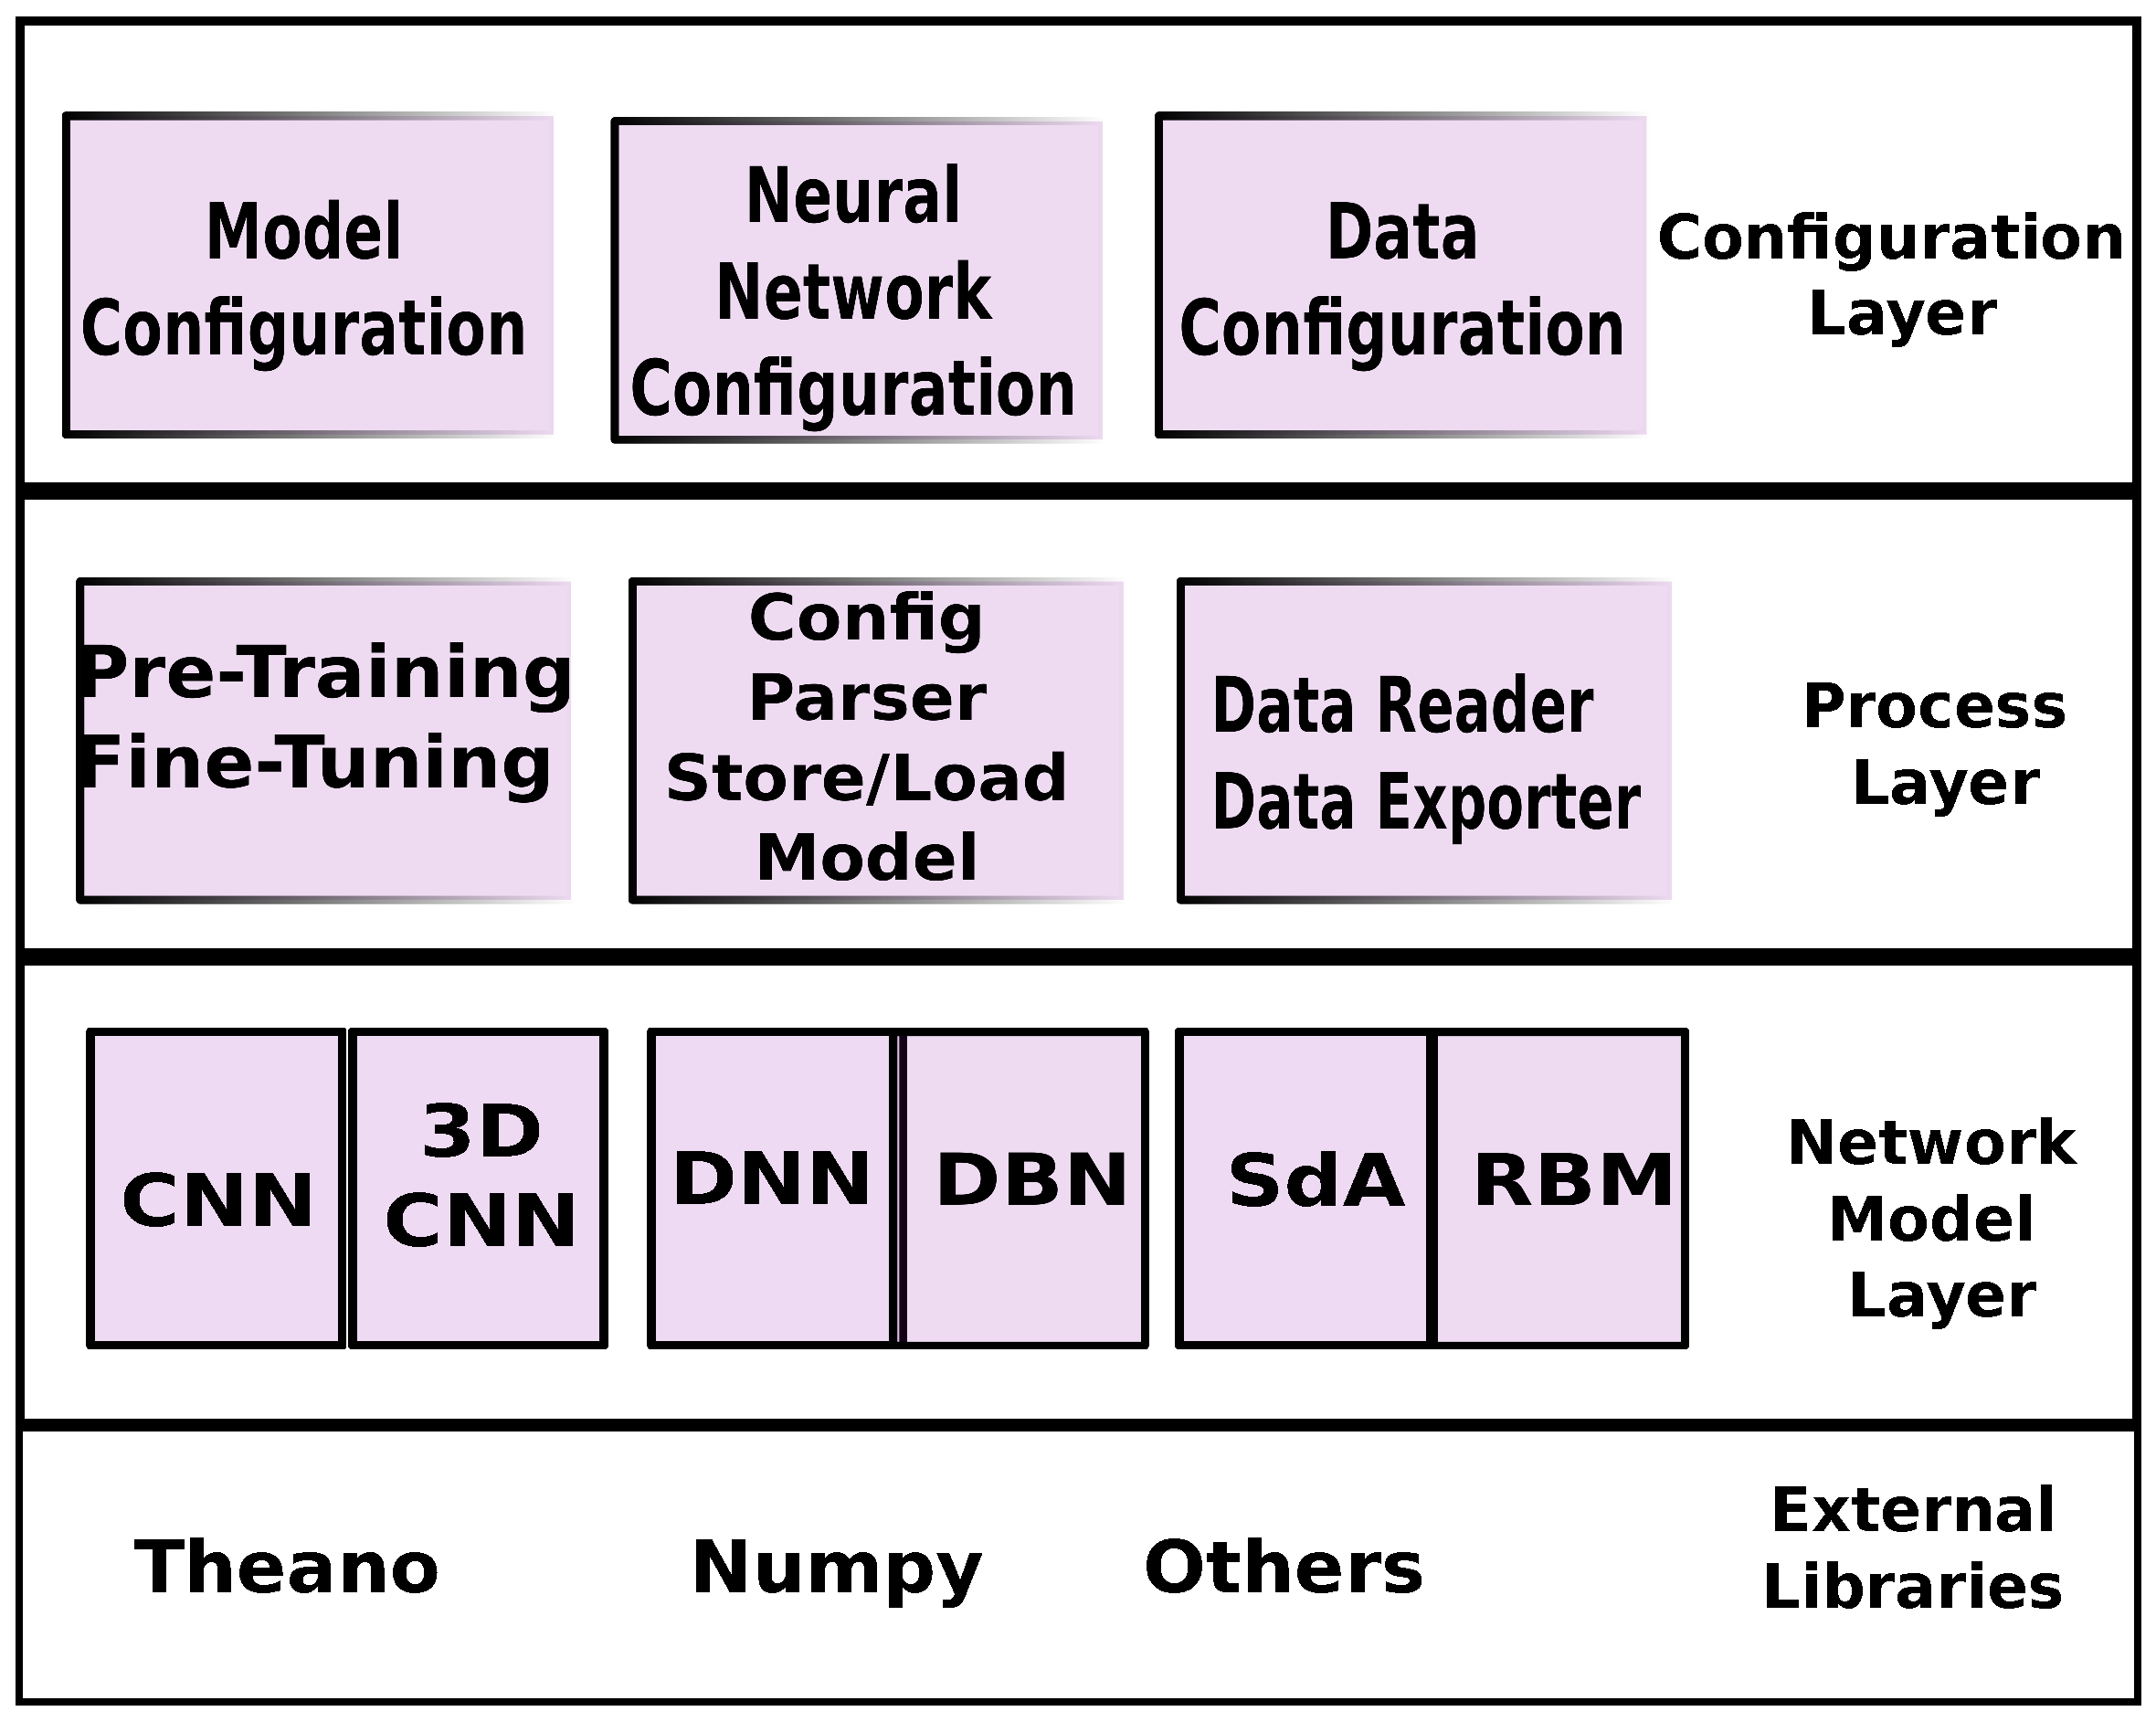
\includegraphics[width=0.7\textwidth]{./imgs/Python-DNNArch.eps}
\caption{Architecture of Python-DNN}
\label{fig:pydnn-arch}
\end{figure}

\textit{Python-DNN} uses \emph{theano} library, which provides an efficient platform for running in both CPU and GPU architectures.  The architecture of our indigenous toolkit is shown on Figure.\ref{fig:pydnn-arch}. 

\noindent The tool-kit can be partitioned into 4 abstract layers:
\begin{itemize}
\item The \textit{external libraries} that include all the dependent libraries
\item The \textit{Network model layer} contains different supervised and unsupervised models.
\item Different operations on different models are performed by \textit{processing layer}
\item The \textit{configuration layer} specifies all details of the input and model to lower layers.
\end{itemize}

Details of the configuration of the toolkit is given in Appendix \ref{app:pythondnn}

\subsection{Salient Features}
\label{sec:python-dnnFeatures}
\begin{itemize}
\item Easy configuration of the models, configurations
are organised in JSON format and hence are legible.
\item Run efficiently in CPU and GPU architectures.
\item Able to load the pre-trained model and dump the trained model.
\item Different types of data reader and data exporter.
\item Can be used as a standalone application as well as a standard  library.
\item Released under \textit{Apache Software License(version 2)}.\\
\end{itemize}

\section{Summary}
\textit{Python DNN} is an indigenous deep neural network toolkit which is easy to configure and able to make use of both GPU and CPU architectures.  The toolkit is publicly hosted in github\footnote{Public repository of \textit{Python-DNN} : (\url{https://github.  com/IITM-DONLAB/python-dnn})}.  This toolkit was jointly developed with G.~ K.~Sudharshan.

Further details about the toolkit installation, configuration and its usage are explained in Appendix \ref{app:pythondnn}
%%%%%%%%%%%%%%%%%%%%%%%%%%%%%%%%%%%%%%%%%%%%%%%%%%%%%%%%%%%%%%%%%%%%%%%%%%%%%%%%%%%%%%%%%%%%%%%%%%%%%%%%%%%%%%%%%%%%%%%%
